\documentclass[17pt]{report}
\usepackage[utf8]{inputenc}
\usepackage{amsmath}
\usepackage{graphicx}
\usepackage{hyperref}
\usepackage{listings}
\usepackage{color}
\hypersetup{
    colorlinks=true,
    linkcolor=blue,
    filecolor=magenta,      
    urlcolor=cyan,
}
 
\urlstyle{same}
\definecolor{codegreen}{rgb}{0,0.6,0}
\definecolor{codegray}{rgb}{0.5,0.5,0.5}
\definecolor{codepurple}{rgb}{0.58,0,0.82}
\definecolor{backcolour}{rgb}{0.95,0.95,0.92}
\lstdefinestyle{mystyle}{
    backgroundcolor=\color{backcolour},   
    commentstyle=\color{codegreen},
    keywordstyle=\color{magenta},
    numberstyle=\tiny\color{codegray},
    stringstyle=\color{codepurple},
    basicstyle=\footnotesize,
    breakatwhitespace=false,         
    breaklines=true,                 
    captionpos=b,                    
    keepspaces=true,                 
    numbers=left,                    
    numbersep=5pt,                  
    showspaces=false,                
    showstringspaces=false,
    showtabs=false,                  
    tabsize=2
}
\lstset{style=mystyle}
\graphicspath{ {../} }
\title{
	{\large Statistical learning: Second assignment}\\}
\author{Ali Zamani(96123035)}
\begin{document}
\maketitle

\newpage
\section{Visualize dataset}
In this project I use creditcard dataset  The dataset contains transactions made by credit cards in September 2013 by European cardholders over a two day period. There are 492 frauds out of a total 284,807 examples. Thus, the dataset is highly unbalanced, with the positive class (frauds) accounting for only 0.172\% of all transactions. You can imagine that any such dataset would be highly unbalanced, as expected fraud or anomalous cases would only make up for a small percentage of the total transactions. Let's have look at our dataset.
\\
I used seaborn and matplotlib to visualize dataset.
\subsection{Import packages and dataset}
\lstinputlisting[language=python, firstline=1, lastline=21]{../Visualize/Visualize.py}
Output:\\
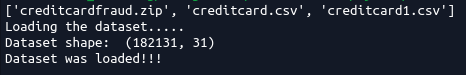
\includegraphics[width=5cm, height=1cm]{/Visualize/import}\\
\subsection{Balance of Data Visualization}
Let's get a visual confirmation of the unbalanced data in this fraud dataset.
\lstinputlisting[language=python, firstline=22, lastline=28]{../Visualize/Visualize.py}
Output:\\
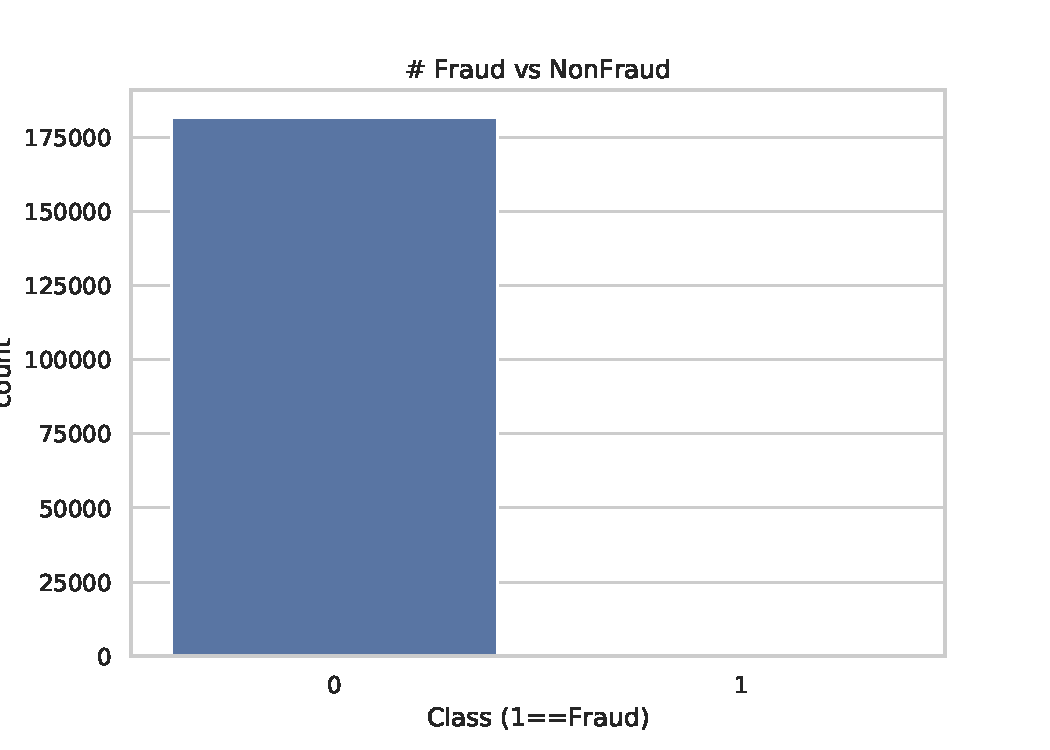
\includegraphics[width=12cm, height=9cm]{/Visualize/fraudvsnonfraud}\\
As you can see, the non-fraud cases strongly outweigh the fraud cases.
\subsection{Heatmap}
\lstinputlisting[language=python, firstline=29, lastline=39]{../Visualize/Visualize.py}
Output:\\
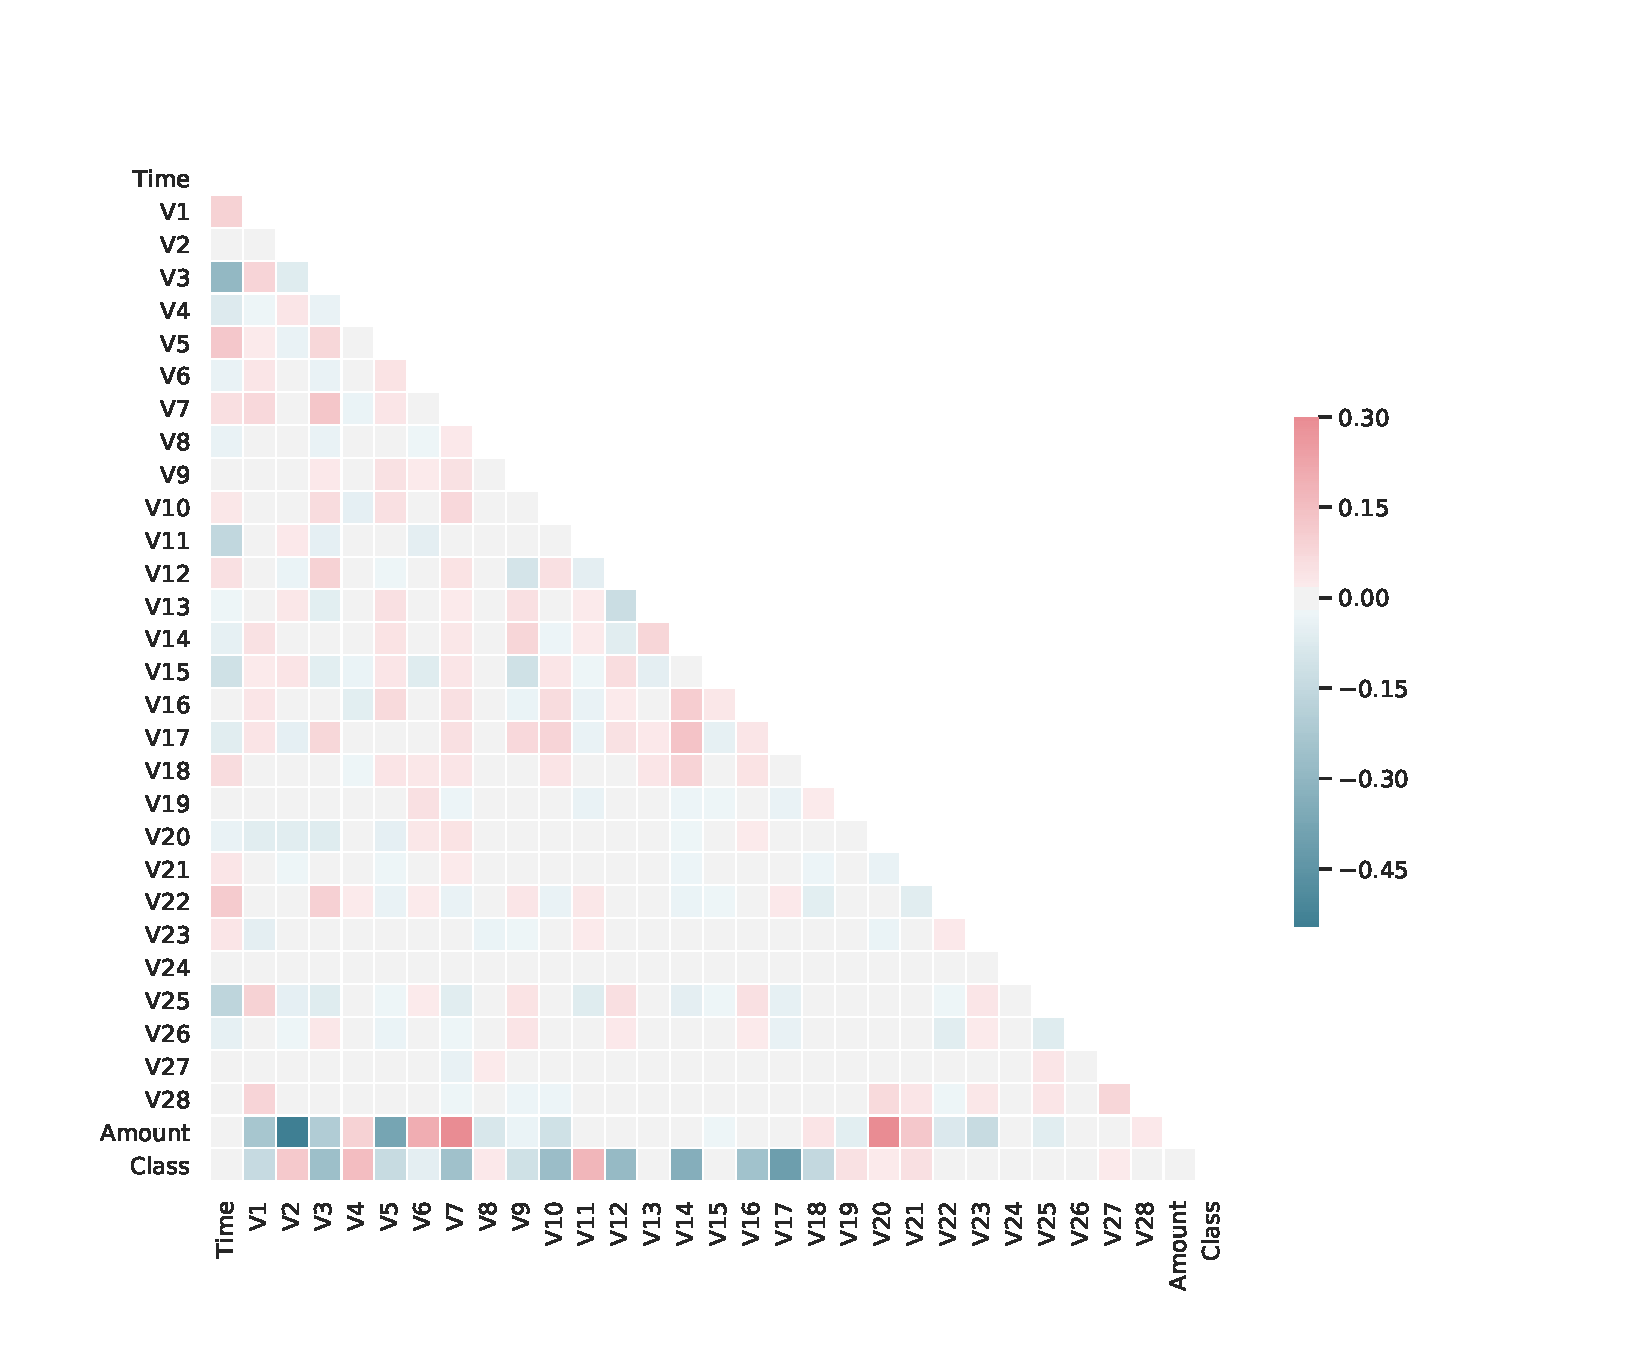
\includegraphics[width=12cm, height=9cm]{/Visualize/heatmap}\\
\subsection{Fraud and non-fraud data describe}
We will cut up the dataset into two data frames, one for non-fraud transactions and the other for fraud.\\
\lstinputlisting[language=python, firstline=40, lastline=42]{../Visualize/Visualize.py}
Let's look at some summary statistics and see if there are obvious differences between fraud and non-fraud
transactions.\\
\lstinputlisting[language=python, firstline=43, lastline=43]{../Visualize/Visualize.py}
Output:\\
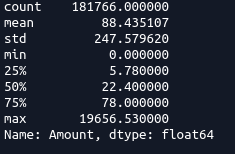
\includegraphics[width=5cm, height=2cm]{/Visualize/NonfraudAmount}\\
\lstinputlisting[language=python, firstline=44, lastline=44]{../Visualize/Visualize.py}
Output:\\
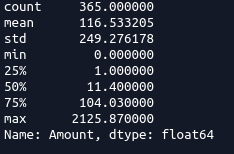
\includegraphics[width=5cm, height=2cm]{/Visualize/fraudAmount}\\
Although the mean is a little higher in the fraud transactions, it is certainly within a standard deviation and so is
unlikely to be easy to discriminate in a highly precise manner between the classes with pure statistical methods.
I could run statistical tests (e.g. t-test) to support the claim that the two samples likely come from populations
with similar means and deviations. However, such statistical methods are not the focus of this article on
autoencoders.
\subsection{Visual Exploration of the Transaction Amount Data}
We are going to get more familiar with the data and try some basic visuals. In anomaly detection datasets it is
common to have the areas of interest "washed out" by abundant data. The most common method is to simply
'slice and dice' the data in a couple different ways until something interesting is found. Although this practice is
common, it is not a scientifically sound way to explore data. There are always non-meaningful quirks to real
data, so just looking until you "find something interesting" is likely going to result in you finding false positives.
In other words, you find a random pattern in the current data set that will never be seen again. As a
famous economist wrote, "If you torture the data long enough, it will confess."\\
In this dataset, I expect a lot of low-value transactions that will be generally uninteresting (buying cups of coffee,
lunches, etc). This abundant data is likely to wash out the rest of the data, so I decided to look at the data in a
number different \$100 and \$1,000 intervals. Since it would be tedious to show reader these graphs, I will only
show the final graph that only visualizes the transactions above \$200.\\
\lstinputlisting[language=python, firstline=45, lastline=54]{../Visualize/Visualize.py}
Output:\\
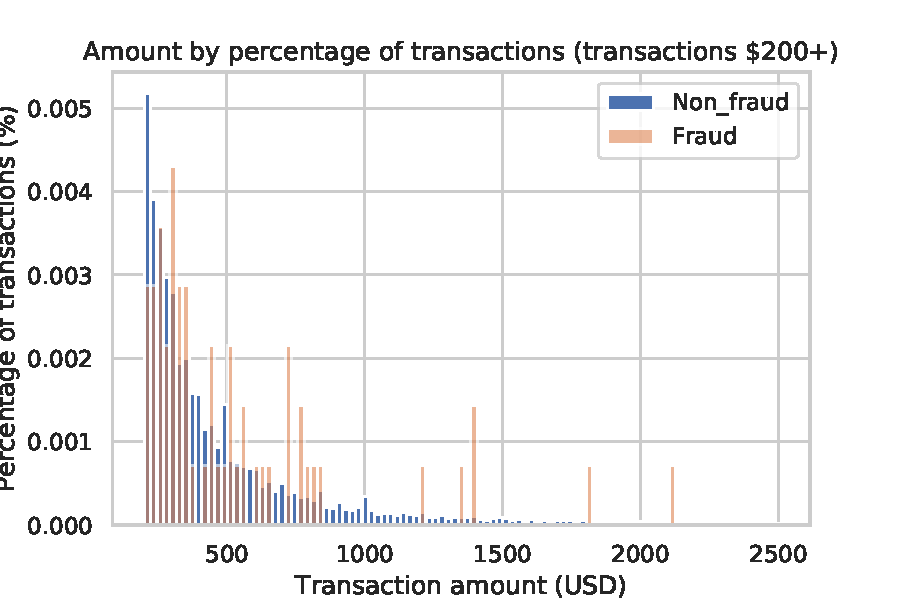
\includegraphics[width=12cm, height=9cm]{/Visualize/Amountbypercentageoftransactions}\\
Since the fraud cases are relatively few in number compared to bin size, we see the data looks predictably more
variable. In the long tail, especially, we are likely observing only a single fraud transaction. It would be hard to
differentiate fraud from non-fraud transactions by transaction amount alone.
\subsection{Visual Exploration of the Data by Hour}
With a few exceptions, the transaction amount does not look very informative. Let's look at the time of day next.\\
\lstinputlisting[language=python, firstline=55, lastline=64]{../Visualize/Visualize.py}
Output:\\
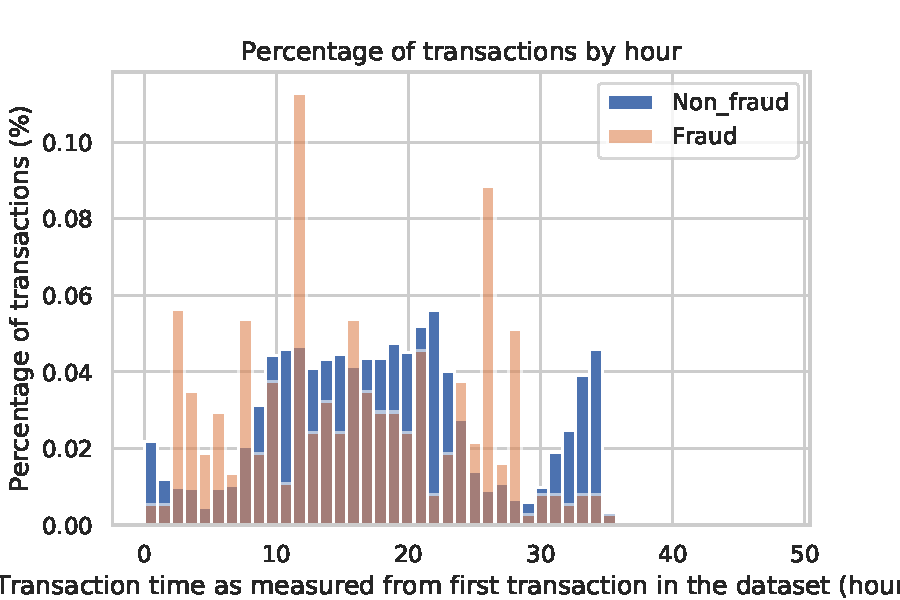
\includegraphics[width=12cm, height=9cm]{/Visualize/VisualExplorationoftheDatabyHour}\\
Hour "zero" corresponds to the hour the first transaction happened and not necessarily 12-1am. Given the
heavy decrease in non-fraud transactions from hours 1 to 8 and again roughly at hours 24 to 32, I am assuming
those time correspond to nighttime for this dataset. If this is true, fraud tends to occur at higher rates during the
night. Statistical tests could be used to give evidence for this fact, but are not in the scope of this article. Again,
however, the potential time offset between normal and fraud transactions is not enough to make a simple,
precise classifier.
Next, we will explore the potential interaction between transaction amount and hour to see if any patterns
emerge.
\subsection{Visual Exploration of Transaction Amount vs. Hour}
\lstinputlisting[language=python, firstline=65, lastline=73]{../Visualize/Visualize.py}
Output:\\
%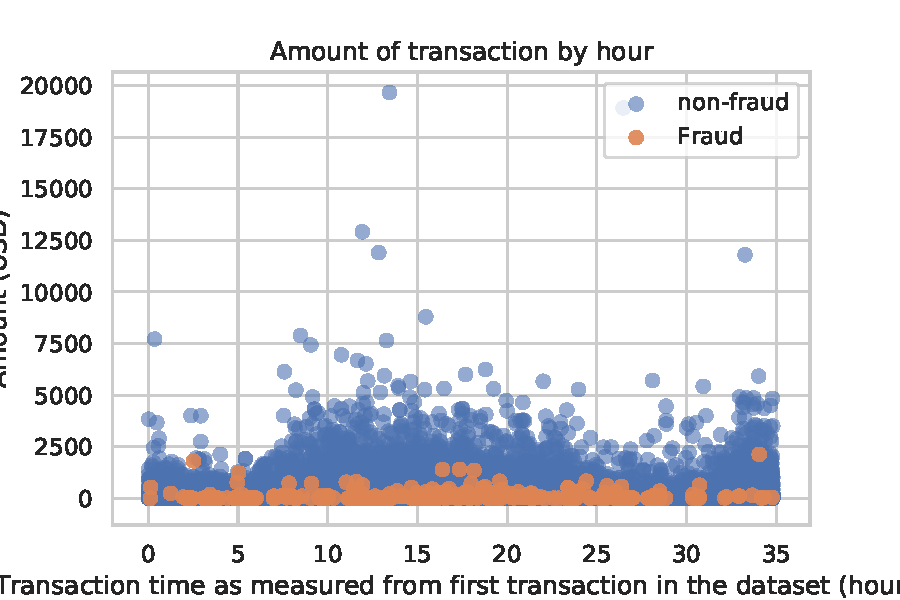
\includegraphics[width=12cm, height=9cm]{/Visualize/VisualExplorationofTransactionAmountvsHour}\\
Again, this is not enough to make a good classifier. For example, it would be hard to draw a line that cleanly
separates fraud and normal transactions. For the experienced Data Scientists in the readership, I am excluding
more advanced techniques such as the kernel trick.\\
\section{Logistic model with sklearn}
\lstinputlisting[language=python]{../LogisticModelwithSklearn/logisticRegression_sklearn.py}
Results:\\
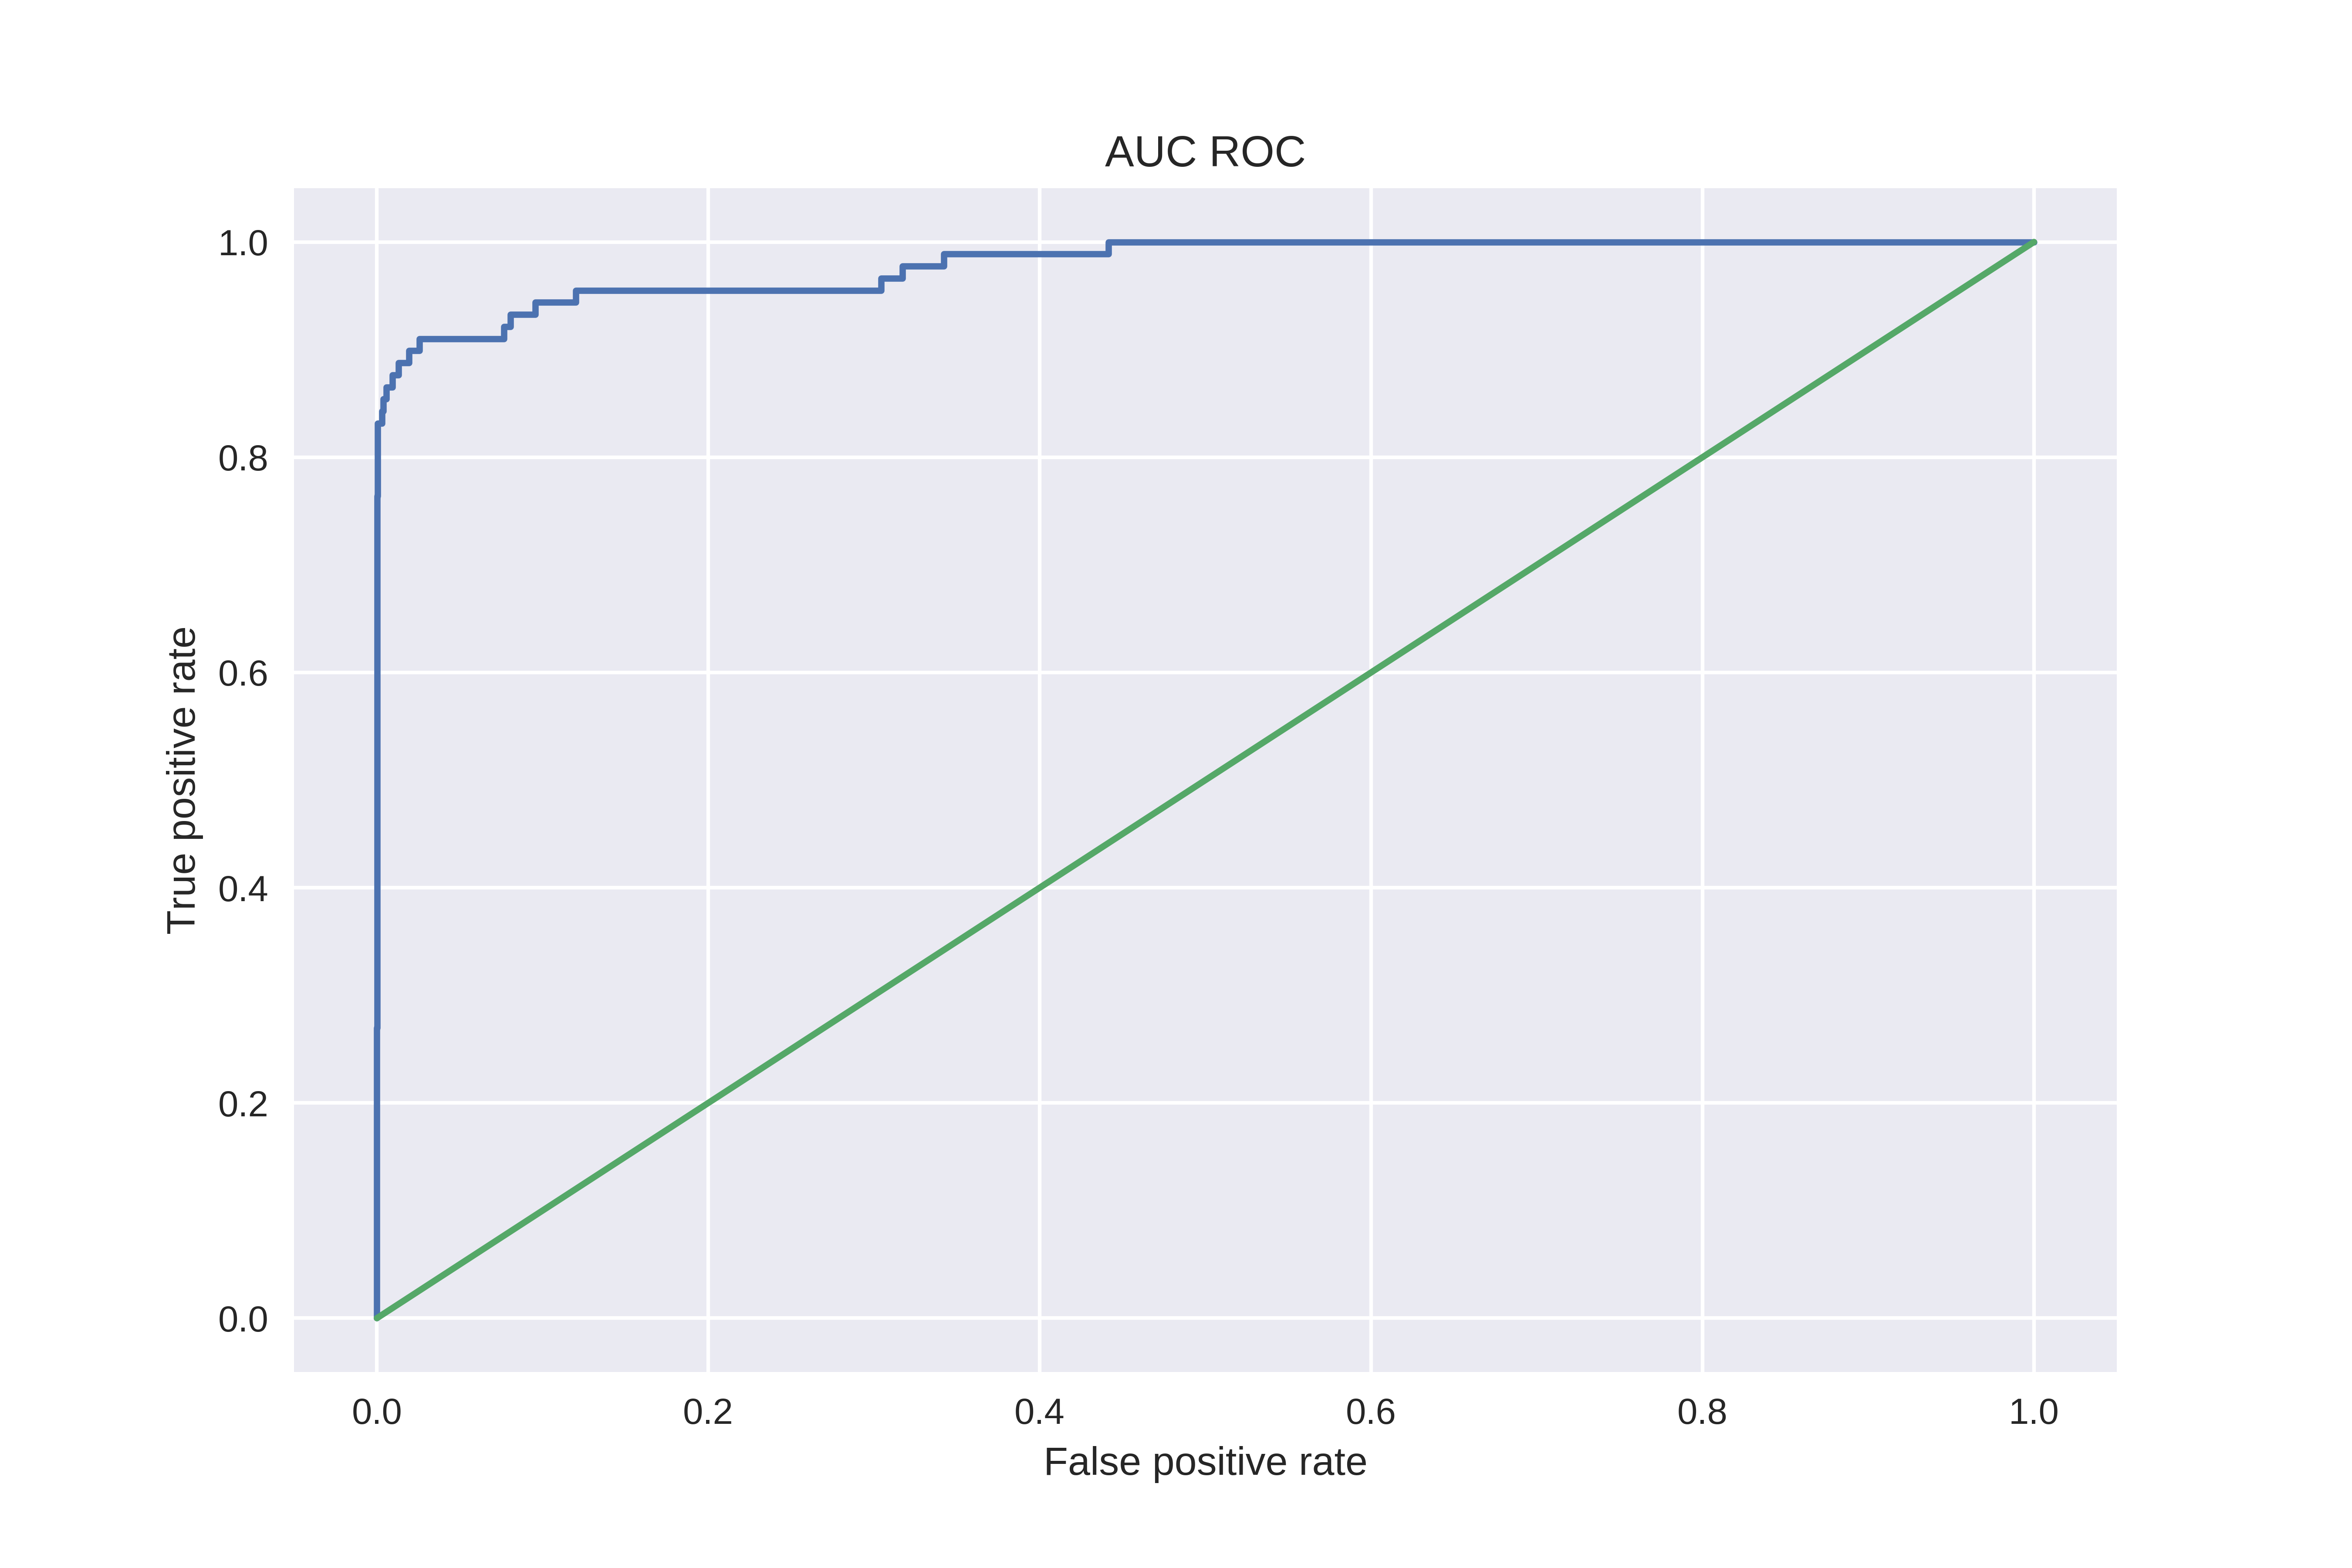
\includegraphics[width=10cm, height=7cm]{/LogisticModelwithSklearn/auc_roc}\\
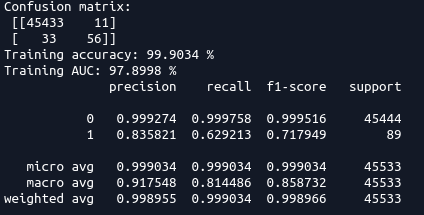
\includegraphics[width=5cm, height=2cm]{/LogisticModelwithSklearn/50}\\
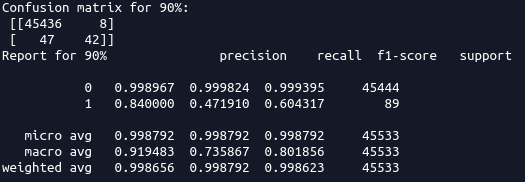
\includegraphics[width=5cm, height=2cm]{/LogisticModelwithSklearn/90}\\
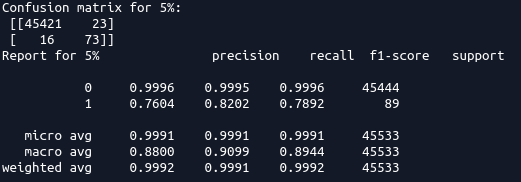
\includegraphics[width=5cm, height=2cm]{/LogisticModelwithSklearn/5}
\section{Logistic model with tensorflow}
\lstinputlisting[language=python]{../Logisticmodelwithtensorflow/logisticRegression_tensorFlow.py}
Results:\\
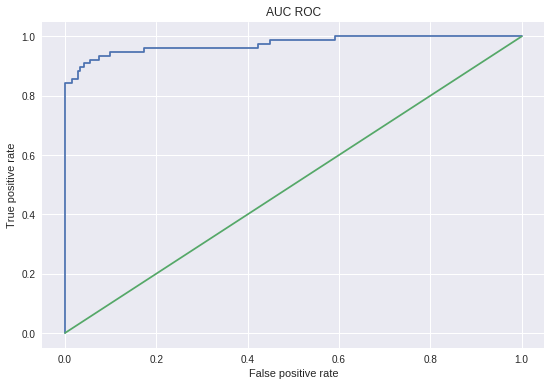
\includegraphics[width=10cm, height=7cm]{/Logisticmodelwithtensorflow/roc}\\
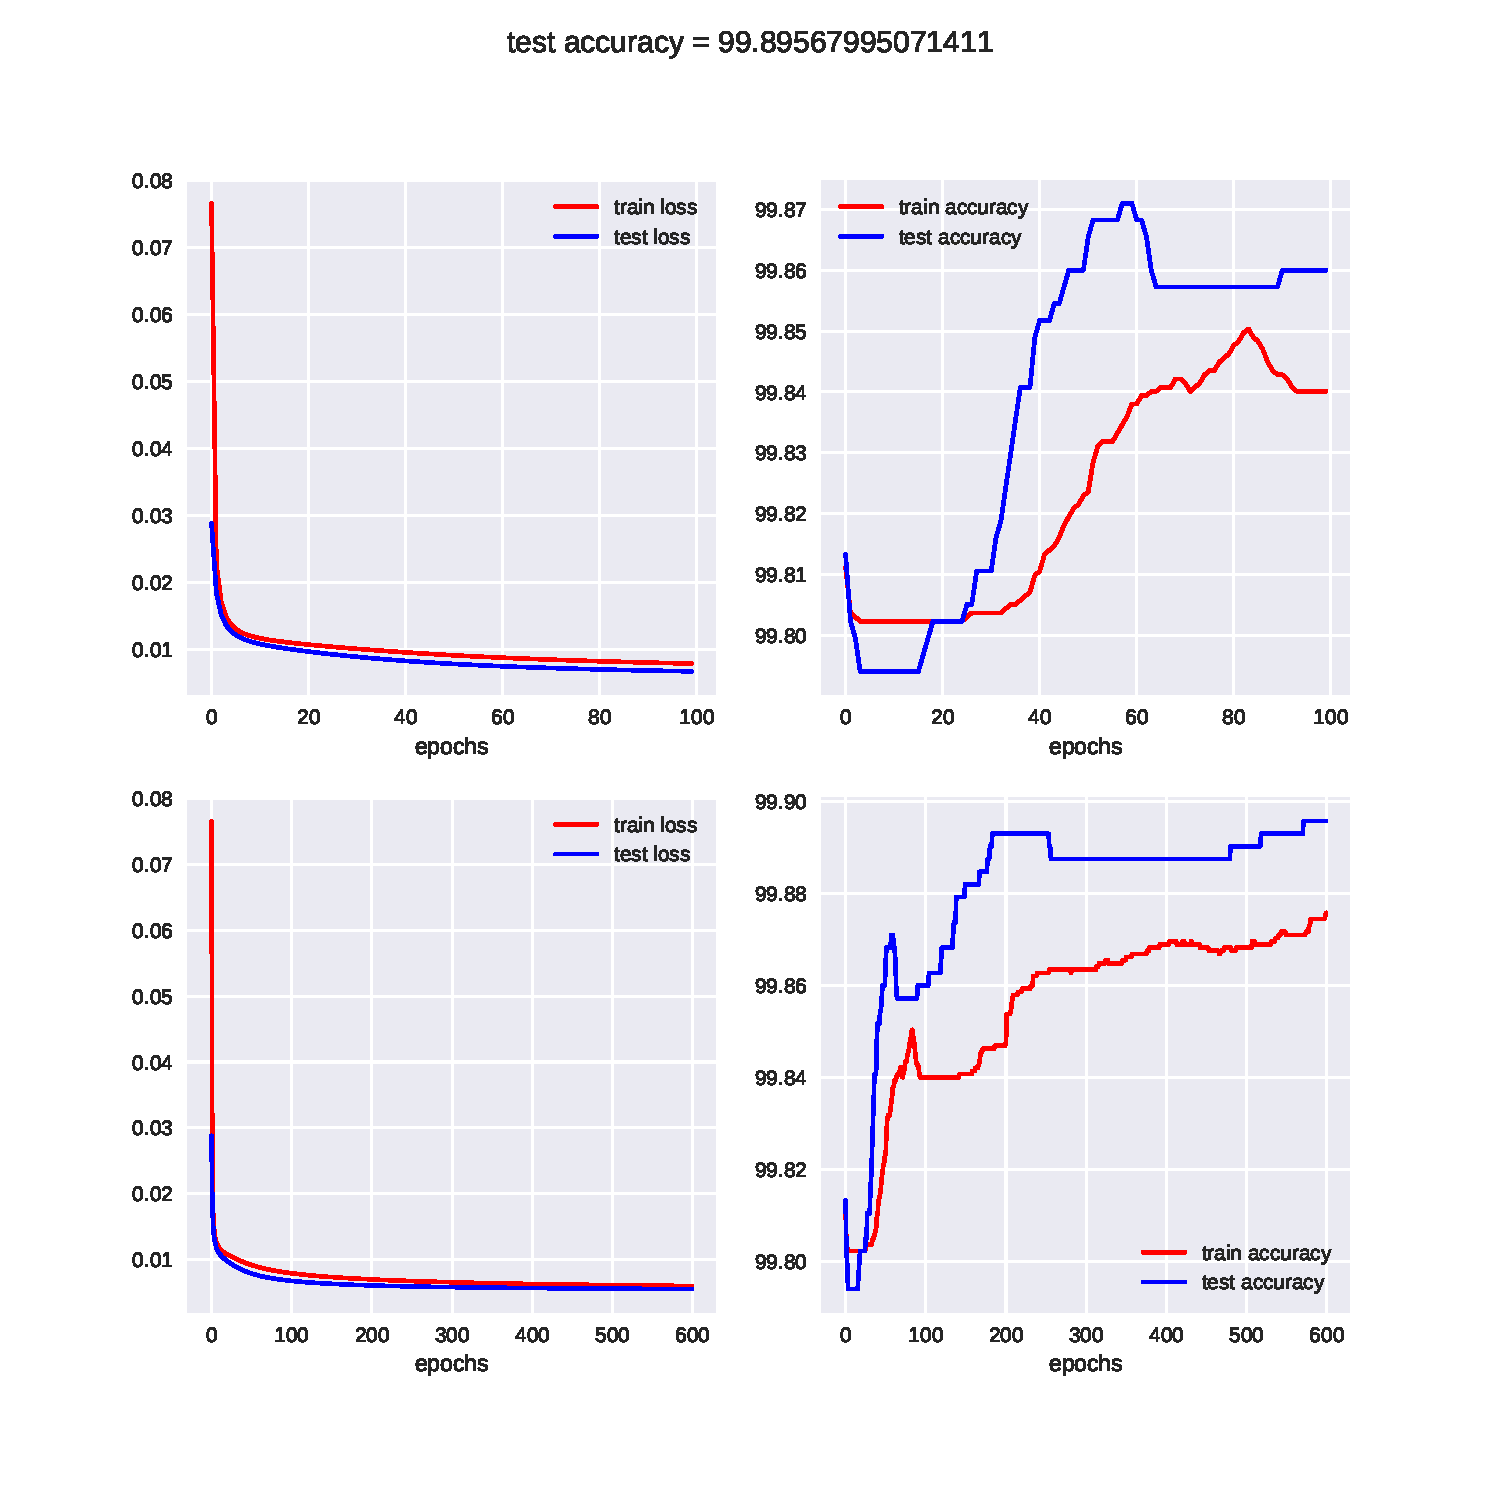
\includegraphics[width=15cm, height=9cm]{/Logisticmodelwithtensorflow/trainandtest.pdf}\\
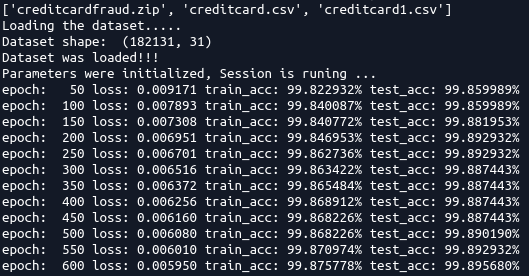
\includegraphics[width=5cm, height=2cm]{/Logisticmodelwithtensorflow/run}\\
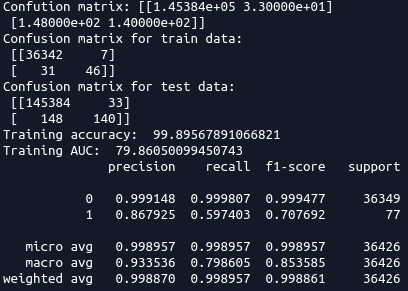
\includegraphics[width=5cm, height=2cm]{/Logisticmodelwithtensorflow/50}\\
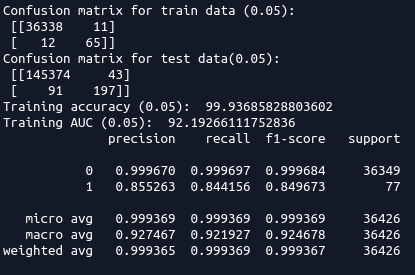
\includegraphics[width=5cm, height=2cm]{/Logisticmodelwithtensorflow/5}
\section{compare sklearn and tensorflow results for logistic model}
Accuracy model of sklearn and tensorflow are  99.9\% and 99.89\% but we know because of unbalance data, accuracy is not suitable criteria hence we compare recall(percentage of one data is fraud and our model predict it fraud) and precision(percentage of one data is non-fraud and our model predicts it non-fraud) and f1-score(recall and precision) of two packages.\\
Recall:\\
sklearn:82\%\\
tensorflow:84\%\\
Precision:\\
sklearn:76\%\\
tensorflow:85\%\\
F1-score:\\
sklearn:79\%\\
tensorflow:85\%\\  
We see that tensorflow predict better.
\section{SVM with sklearn}

\section{SVM with tensorflow}
	
\section{Compare sklearn and tensorflow results for SVM}

\end{document}